\documentclass[varwidth, border=5pt]{standalone}

% Inspiration:
% https://www.mdpi.com/information/information-11-00557/article_deploy/html/images/information-11-00557-g001.png
%
% See also:
% https://tex.stackexchange.com/questions/518863/

\usepackage[utf8]{inputenc}
\usepackage[T1]{fontenc}
\usepackage{tikz}
\usepackage{amsmath}
\usetikzlibrary{calc, positioning}

\begin{document}

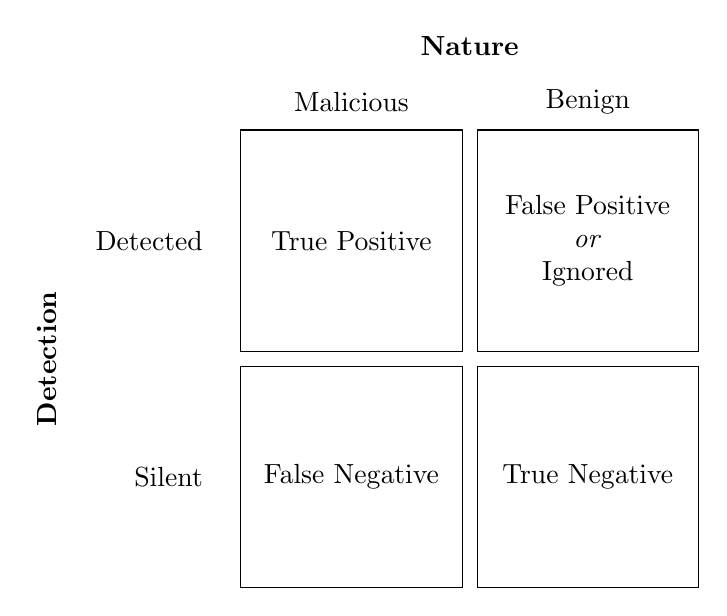
\begin{tikzpicture}[
  cell/.style={minimum width=8em, minimum height=8em, draw, align=center},
  label/.style={font=\normalsize},
  total/.style={font=\normalsize},
  boxgap/.style={xshift=1em, yshift=-1em}
]

% Define matrix blocks
\node[cell] (TP) at (0,0) {True Positive};
\node[cell, right=0.5em of TP] (FN) {False Positive\\\emph{or}\\Ignored};
\node[cell, below=0.5em of TP] (FP) {False Negative};
\node[cell, right=0.5em of FP] (TN) {True Negative};

% Axis labels
\node[label, rotate=00] at ([yshift=3em]$(TP.north)!0.5!(FN.north)$) {\textbf{Nature}};
\node[label, rotate=90] at ([xshift=-7em]$(TP.west)!0.5!(FP.west)$)  {\textbf{Detection}};

% Individual cell axis labels
\node[label, anchor=center] at ([yshift=1em]TP.north) {Malicious};
\node[label, anchor=center] at ([yshift=1em]FN.north) {Benign};
\node[label, anchor=east] at ([xshift=-1em]TP.west) {Detected};
\node[label, anchor=east] at ([xshift=-1em]FP.west) {Silent};

\end{tikzpicture}

\end{document}